% Template for IGARSS-2020 paper; to be used with:
%          spconf.sty  - LaTeX style file, and
%          IEEEbib.bst - IEEE bibliography style file.
% --------------------------------------------------------------------------
\documentclass{article}
\usepackage{spconf,amsmath,epsfig}
\usepackage{dblfloatfix}
\usepackage{makecell}
\usepackage{multirow}
\usepackage{booktabs}
\usepackage{subfigure}
\usepackage{graphicx}
%\usepackage[backend = biber, sytle = nwsuafref, utf8, sorting = centy]{biblatex}
%\addbibresource{myrefs}

% Example definitions.
% --------------------
\def\x{{\mathbf x}}
\def\L{{\cal L}}

% Title.
% ------
\title{An Extreme Learning Machine Correction Network for High Precision Satellite Attitude Determination}
%
% Single address.
% ---------------
\name{Kailang Cao, Jiaojiao Li, Rui Song, Yunsong Li, Weijiao Jiang\thanks{This work was supported in part by the National Defense Science and Technology Key Laboratory Fund(No.6142411184413), in part by the National Nature Science Foundation of China(No.61901343), in part by Science and Technology on Space Intelligent Control Laboratory(No.ZDSYS-2019-03).}}
\address{State Key Laboratory of Integrated Services Networks, Xidian University, Xi'an, China}
%
% For example:
% ------------
%\address{School\\
%	Department\\
%	Address}
%
% Two addresses (uncomment and modify for two-address case).
% ----------------------------------------------------------
%\twoauthors
%  {A. Author-one, B. Author-two\sthanks{Thanks to XYZ agency for funding.}}
%	{School A-B\\
%	Department A-B\\
%	Address A-B}
%  {C. Author-three, D. Author-four\sthanks{The fourth author performed the work
%	while at ...}}
%	{School C-D\\
%	Department C-D\\
%	Address C-D}
%
	\begin{document}
	%\ninept
	%
	\maketitle
	%
	\begin{abstract}
	The fusion framework of star sensor and gyro based on adaptive Kalman filter is widely used in satellite pose estimation. However, the discretization and linearization inevitably introduce system errors, which degrades of the filtering accuracy. To address this problem, we propose a high-precision satellite attitude determination algorithm based on extreme learning machine network correction. We design a dedicated network for error compensation and trained the parameters effectively. In attitude calculation procedure, the forward fusion filtering of star sensor and gyro data is performed firstly by using the adaptive Kalman filter. Then the filtering estimation results are compensated by the extreme learning machine network proposed in this paper. After that, backward smoothing is performed to solve the high-precision attitude. Simulation results show that armed with the compensation procedure of the proposed extreme learning machine network, the accuracy of estimated pose is significantly improved.
	\end{abstract}
%
	\begin{keywords}
		Extreme learning machine, Satellite attitude, star sensor/gyro,  combined attitude determination, adaptive Kalman filter
	\end{keywords}
	%
	
	\section{Introduction}
	\label{sec:intro}	
	Recently, according to the demand of geospatial information for national defense and social development, high precise mapping technology is one of the main tasks of aerospace remote sensing mapping. The accuracy of the stereo mapping satellite system depends on the performance of the on-board camera and system sensors, among which, the satellite attitude information is an important factor of the positioning accuracy of the stereo mapping satellite.
	
	Gyroscopes and star sensors are common combinations that constitute the attitude determination system of stereo mapping satellites\cite{hou2019integrated}. 
	The effective fusion of the sensors' measurement informationis the main way for the current high-precision combined attitude determination, which can overcome their respective shortcomings.
	
	The classical combined satellite attitude determination algorithm uses the Kalman filter as the key framework. Based on this algorithm basis, researchers have also continued to propose various improvement methods. C.Hajiyev\cite{hajiyev2015integration} proposed an extended Kalman filter based on the algebraic method, which is suitable for scenarios with increasing measurement error covariance matrix.
	%LI You et al [] proposed a combined attitude determination algorithm based on the minimum model error for modeling spatial disturbances and system model errors, the model estimated values is fused into the EKF algorithm to improve the accuracy. 
	%To address the shortcomings of the EKF algorithm with low estimation accuracy and poor stability, JI Xiaoqin et al [] proposed an inertial navigation system attitude determination method based on modified Rodriguez parameters, which constructs the system model in the inertial framework and uses UKF for filtering. The attitude results can converge to ${0.01^ \circ }$. 
	C. Guo et al.\cite{guo2017high} proposed a unscented Kalman filtering algorithm with complementary filter. The attitude data based on complementary filtering is introduced as the measurement value of UKF, solve the problem of slow convergence of extended Kalman filter (EKF). 
	Gordon\cite{risfic2004beyond}, Z. Fan\cite{zhiru2013research} applied particle filtering (PF) to combined satellite attitude determination, and compared with EKF and UKF, PF improves the estimation accuracy and algorithm convergence speed when the measurement noise is non-Gaussian distributed.
	
	However, there is a trade-off between computational cost and accuracy in the Kalman filter framework. In order to reduce the approximation error of linear filtering frameworks such as EKF for nonlinear systems, obtain better filtering results with less computational effort, and achieve a higher accuracy attitude determination algorithm, this paper proposes a high-precision satellite attitude determination method based on Extreme Learning Machine (ELM) network correction.
	
	\section{Proposed Method}
	\label{sec:method}	
	
	The main idea of EKF is to use the Taylor series to linearize the approximation of the nonlinear system function. The linearization will not increase the computational cost, which is suitable to solve the estimation problem in practical systems\cite{farhangian2020accuracy}.
	
	Since both the state model and the measurement model are nonlinear functions, the EKF performs linearization at each tiny moment. Because of the Taylor expansion and first-order approximation of the nonlinear state and observation equations, only the Jacobi matrix is retained and the higher order terms are discarded, which causes a systematic error in the EKF. On the one hand, this systematic error will increase with the noise of the attitude sensor data, and on the other hand, it is affected by the level of system nonlinearization.
	
	The existing linear filtering algorithms, such as AEKF\cite{nayak2016comparative}, MEKF\cite{sola2017quaternion}, etc., all consider the uncertainty of attitude measurement error characteristics and the difference between the predicted and measured attitude, so that the attitude error in the filtering process can be better corrected. However, the problem of nonlinear approximation has not been improved, resulting in the attitude results always have a certain gap with the real value. Although nonlinear filtering algorithms such as UKF and PF can achieve good results in approximating nonlinear systems, they bring a huge computational cost, making the overall efficiency of the algorithm inferior to that of linear filtering
	
	\subsection{The Proposed Framework}
	\label{sec:2.2.1}
	The flowchart of the proposed ELM network correction based satellite high precision attitude determination algorithm is shown in Fig.\ref{fig:flowchart}.
	
	In the forward process, the calculation of the incremental quaternion is first performed and the pose estimate at the moment is predicted. Subsequently, the time update step and the measurement update step are performed according to the AEKF algorithm, and the correction of the measurement noise covariance matrix is completed to update the measurement noise prediction characteristics in the filter system. Then, the key parameters of the AEKF filtering process are input to the offline training model of the extreme learning machine network for online prediction, and the attitude compensation amount $\Delta {q_{ELM}}$ is obtained. Then, calculate the state estimation $ {\hat X_{k,ELM}} = {\left[{\begin{array}{*{20}{c}} {\Delta {{\hat q}_{k,ELM}}^T}&{\Delta {b_k}^T} \end{array}} \right]^T} $, where $ \Delta {\hat q_{k,ELM}} = \Delta {\hat q_k} \otimes \Delta {q_{ELM}} $, $ \Delta {b_k} $ is the gyro drift.
	
	In the backward process, the RTS smoothing in k time is first performed to obtain the state smoothing value $ {\hat X'_k} $ and the covariance matrix smoothing value $ {\hat P'_k} $, and then the k moment pose is corrected to obtain high-precision value $ {\hat q'_k} $.
	
	The high-precision satellite attitude determination algorithm based on ELM correction uses the Forward-Backward Adaptive Extended Kalman Filter (FB-AEKF) as the basic framework, which consisting of a forward AEKF and a backward RTS smoother.
	
	\begin{figure}[h]
		\centering
		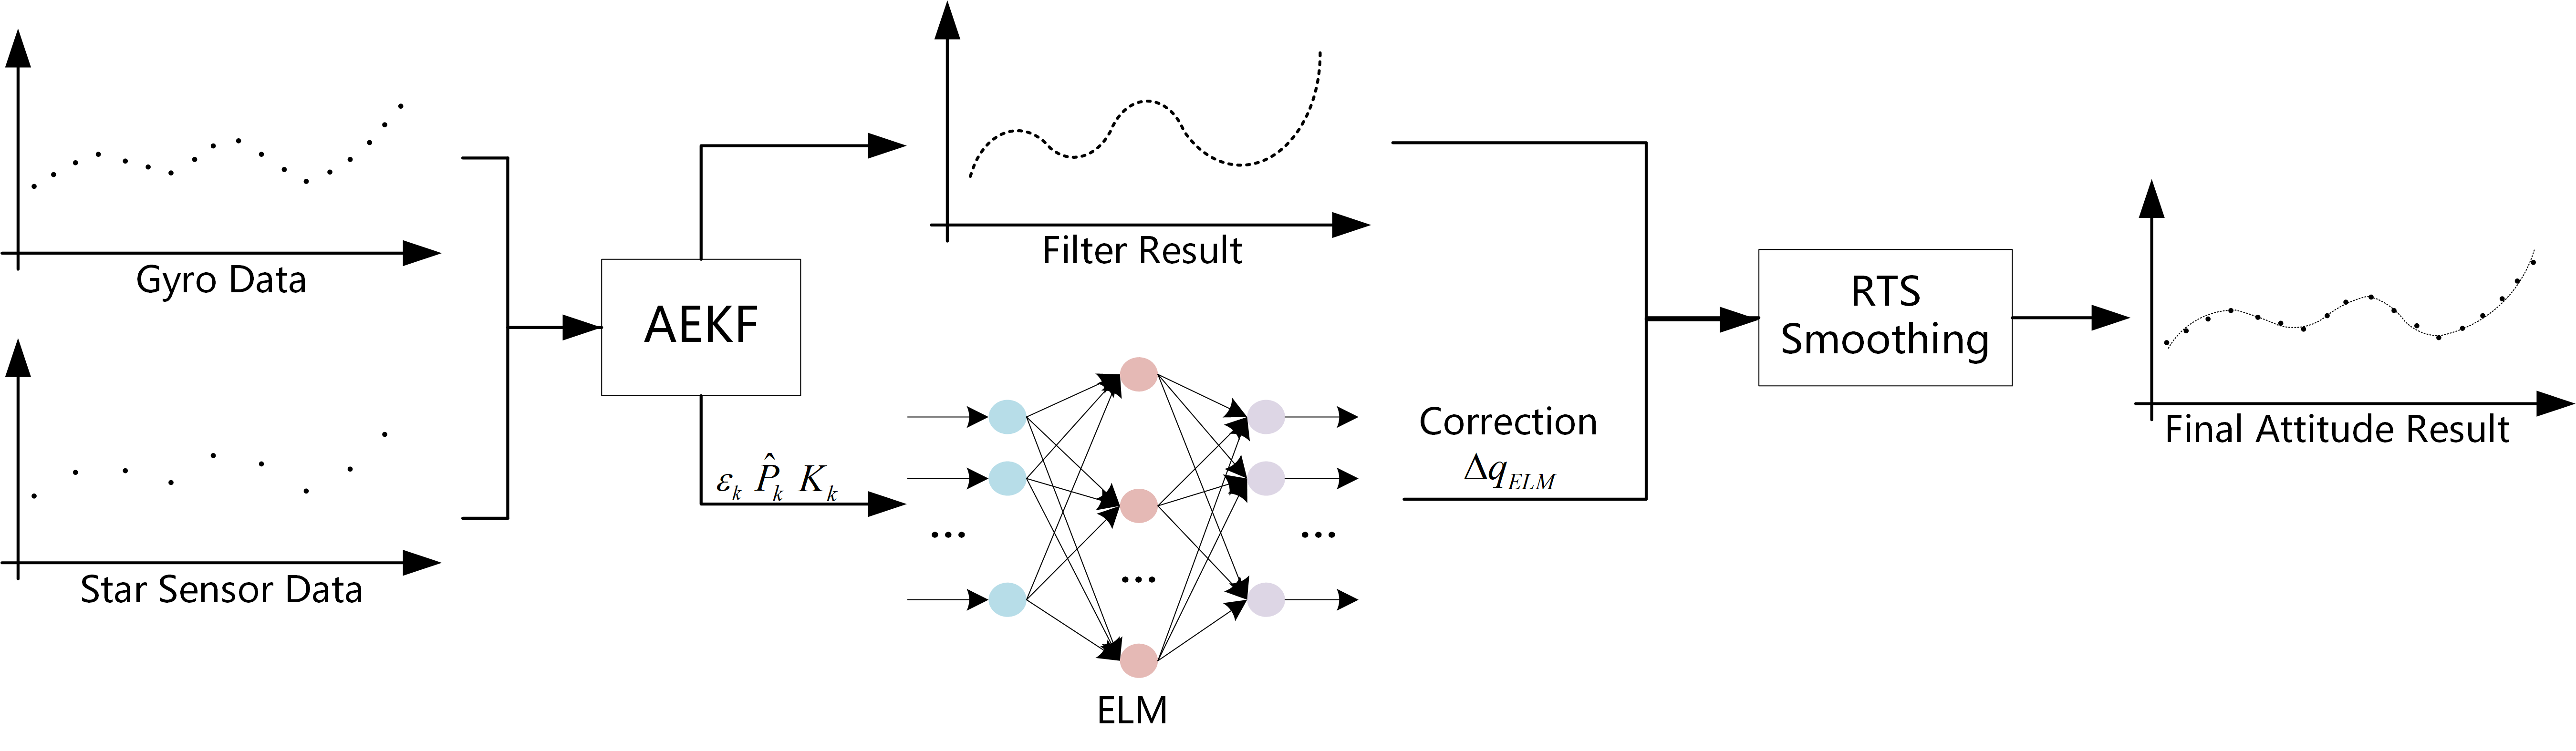
\includegraphics[width=\linewidth]{pic/flowchart1.png}
		\caption{The flowchart of our proposed method}
		\label{fig:flowchart}
	\end{figure}
	
	\subsection{The ELM-based System Error Compensation Model}
	\label{sec:2.2.2}
	Error compensation can be abstracted as a nonlinear mapping problem. There are many factors affecting the filter error, and it is difficult to construct the theoretical nonlinear mathematical equations. Artificial neural network (ANN) is an effective method to deal with complex nonlinear mapping problems. ELM is a single-layer feedforward neural networks (SLFNs), which only need to adjust the number of hideen neurons when used, and has fewer training parameters and faster learning speed\cite{huang2011extreme}. 
	
	According to the framework of forward-backward adaptive extended Kalman filtering, we expect that ELM can learn from the training data the linearization loss in the filtering process, to obtain the difference $ {q_{AKF}}^{ - 1} \otimes {q_{real}} $ between the solved pose quaternions $ {q_{AKF}} $ and the true value of the quaternions $ {q_{real}} $ , i.e., the pose compensation amount $ \Delta {q_{ELM}} $. In the attitude estimation process of AEKF, the nonlinear system error mainly comes from the prediction process of the state covariance matrix $ {P_k} $, and the resulting error will be introduced into the pose estimate through the system residuals ${\varepsilon _k}$ , and the filtering gain $ {K_k} $. Therefore, there is a nonlinear mapping relationship between ${\varepsilon _k}$, $ {P_k} $, $ {K_k} $ and $ \Delta {q_{ELM}} $.
	
	Accordingly, we designed the input quantities of the ELM network as: system residuals: ${\varepsilon _k} = {Y_k} - {H_k}{\mathord{\buildrel{\lower3pt\hbox{$\scriptscriptstyle\frown$}} \over X} _{k,k - 1}}$; state covariance matrix estimates: $ {\hat P_k}{\rm{ = }}\left( {{I_{N \times N}} - {K_k}{H_k}} \right){\mathord{\buildrel{\lower3pt\hbox{$\scriptscriptstyle\frown$}} 	\over P} _{k,k - 1}} $; filtering gain: $ {K_k}{\rm{ = }}{\mathord{\buildrel{\lower3pt\hbox{$\scriptscriptstyle\frown$}} 
			\over P} _{k,k - 1}}{H_k}^T{\left[ {{H_k}{{\mathord{\buildrel{\lower3pt\hbox{$\scriptscriptstyle\frown$}} 
						\over P} }_{k,k - 1}}{H_k}^T + {{\hat R}_k}} \right]^{ - 1}} $, 
	while the output quantity of the network is the pose compensation quantity $\Delta {q_{ELM}}$. (Here, $ I $ is the identity matrix, $ H $ is the Jacobi matrix of nonlinear measurement model.)
	
	\begin{figure}
		\centering
		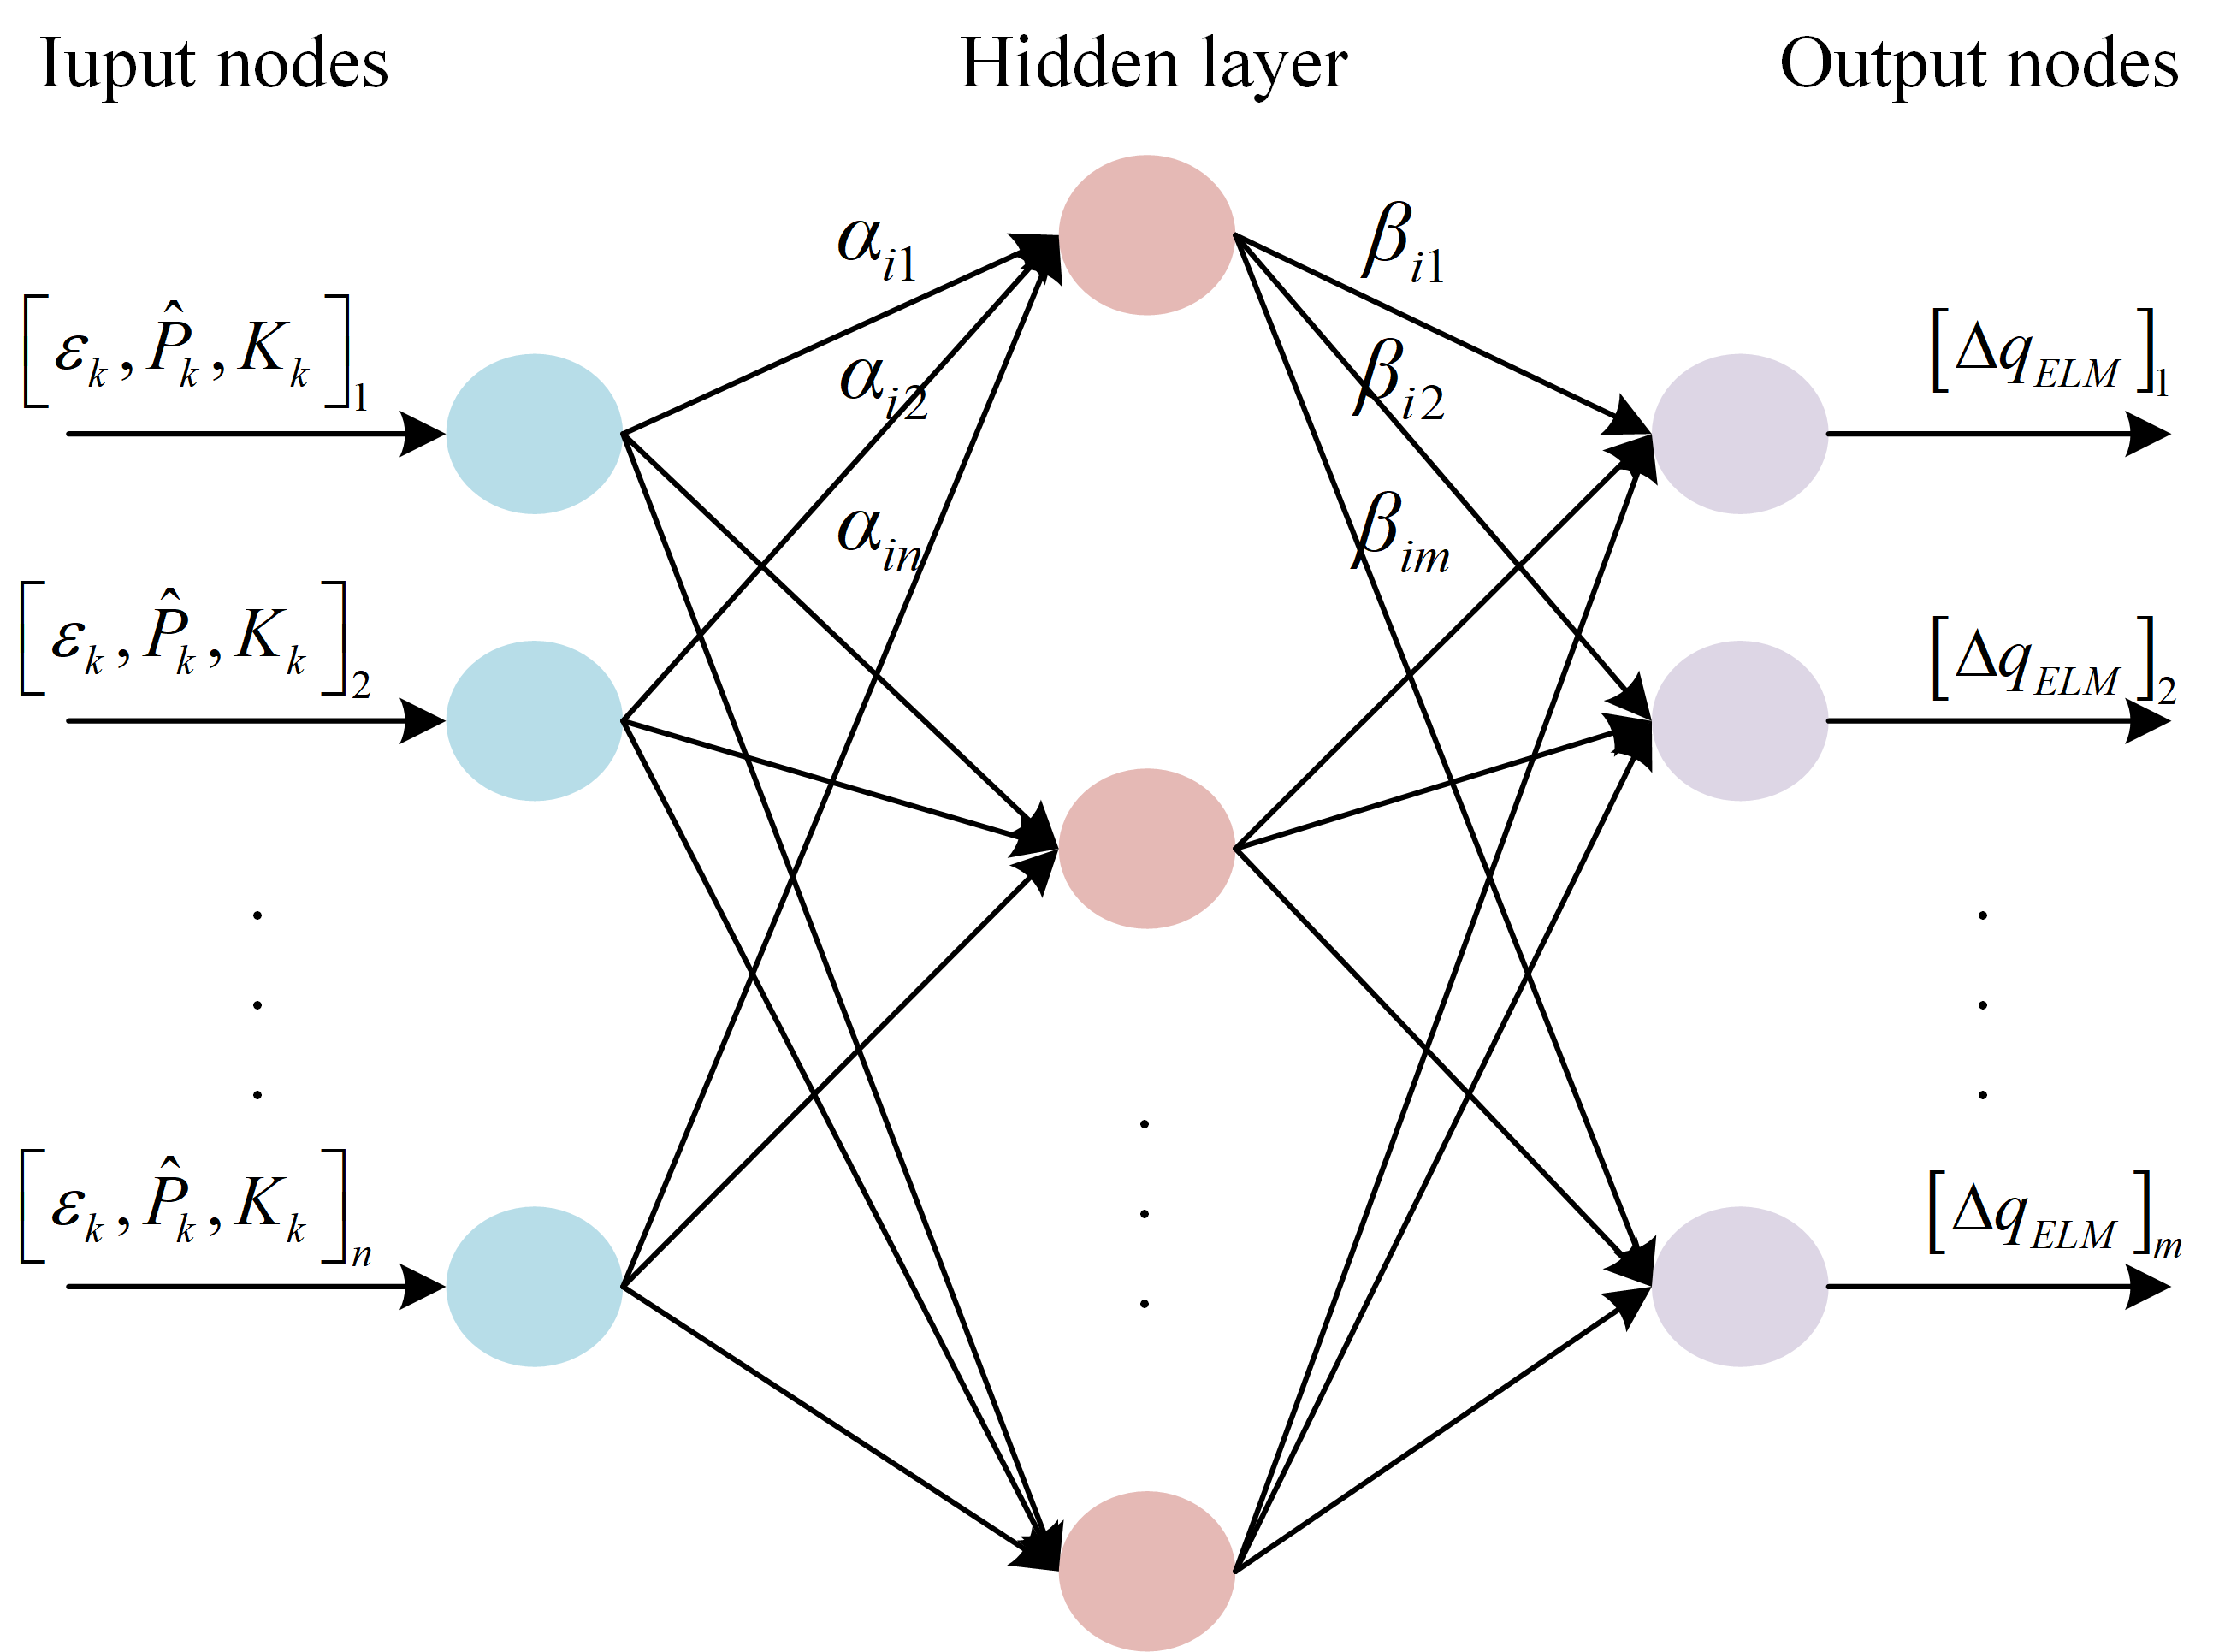
\includegraphics[width=0.8\linewidth]{pic/ELMnetwork1.png}
		\caption{ELM network basic architecture}
		\label{fig:elmnetwork}
	\end{figure}
	
	As shown in Fig.\ref{fig:elmnetwork}, suppose we are given a set of different AEKF filtering parameters $ \left\{ {\left. {\left( {{{\bf{s}}_j},{{\bf{p}}_j}} \right)} \right|j = 1,2, \ldots ,N} \right\} $, where $ {{\bf{s}}_j} = \left\{ {{{\left[ {{\varepsilon _k},{{\hat P}_k},{K_k}} \right]}_{1j}}, \ldots ,{{\left[ {{\varepsilon _k},{{\hat P}_k},{K_k}} \right]}_{nj}}} \right\} $is the input vector and $ {{\bf{p}}_j} = \left\{ {{{\left[ {\Delta {q_{ELM}}} \right]}_{1j}} \ldots {{\left[ {\Delta {q_{ELM}}} \right]}_{mj}}} \right\} $ is the output vector. We set the hidden layer to contain $L$ neurons, $ {{\mathbf{\alpha }}_i} = {\left[ {{\alpha _i}_1,{\alpha _i}_2, \ldots ,{\alpha _i}_n} \right]^T},i \in \left[ {1,...,L} \right] $ is the input weight connecting the first hidden layer neuron, $ {{\bf{\beta }}_i} = {\left[ {{\beta _i}_1,{\beta _i}_2, \ldots ,{\beta _{im}}} \right]^T},i \in \left[ {1,...,L} \right] $ is the output weight connecting the first hidden layer neuron, the bias on the i-th hidden layer neuron is $ {{\bf{b}}_i} $, and $ g( \cdot ) $ is an appropriate activation function. Here, we choose to use the Sigmoid function as the activation function of the network.	
	
	\subsection{Key parameters refinement method}
	\label{sec:2.2.3}
	As described in Sec.\ref{sec:2.2.2}, we choose the system residuals ${\varepsilon _k}$, the state covariance matrix estimates $ {P_k} $, and the filtering gains $ {K_k} $ as the inputs to the network. If the raw data of ${\varepsilon _k}$, $ {P_k} $, and $ {K_k} $ are directly used as sample inputs, there are two problems: the number of sample dimensions is too large, and Data levels within the matrix can vary by ${10^2}$ to ${10^4}$ orders of magnitude. The usual practice of neural networks is to normalize the data, but the input data selected in this paper are not easy to be normalized, so we propose a method for refining the key parameters.
	
	Considering a matrix whose principal diagonal elements contain the main algebraic features of the matrix, we only keep the main diagonal elements directly related to the pose quaternion and discard the non-main diagonal elements and the main diagonal elements only related to the gyroscopic drift error. The final sample input $ {\bf{s}} $ of the training model is obtained as
	\begin{equation}
	{s_{1 \times 9}} = \left[ {\begin{array}{*{20}{c}}
		{{K_{11}}},{{K_{22}}},{{K_{33}}},{{{\hat P}_{11}}},{{{\hat P}_{22}}},{{{\hat P}_{33}}},{{\varepsilon _1}},{{\varepsilon _2}},{{\varepsilon _3}}
		\end{array}} \right]
	\end{equation}
	
	In the training process, the training data $ {{\bf{s}}_{train}} $ and the real values of quaternions ${q_{real}}$ are taken as input, and model outputs the quaternion compensation values $\Delta {q_{ELM}}$, ELM model parameters $ {{\bf{\alpha }}_i} $, $ {{\bf{\beta }}_i} $, $ {{\bf{b}}_i} $ and the number $ L $ of neurons in the hidden layer. The specific steps are as follows.
	
	1) Setting the number $ L $ of neurons in the hidden layer, the initial values consistent with the input data dimension.
	
	2) Randomize the initialization parameters. Including network input and output, $ {{\bf{\alpha }}_i} $, $ {{\bf{\beta }}_i} $ and hidden layer bias $ {{\bf{b}}_i} $.
	
	3) Calculate the output matrix $ {\bf{G}} $ of the hidden layer and  the output layer weight matrix $ {\bf{B}} $.
	
	4) Calculate the network outputs and obtain the pose compensation $\Delta {q_{ELM}}$. Compensate it into the final result, and calculate the errors. If the requirements are met, parameters $ {{\bf{\alpha }}_i} $, $ {{\bf{\beta }}_i} $, $ {{\bf{b}}_i} $ and $ L $ will output. If not, the number of neurons in the hidden layer is increased and the above steps are repeated.
	
	The test procedure of the system error compensation model based on ELM takes the test data $ {{\bf{s}}_{test}} $ as input and outputs the quadratic compensation value $\Delta {q_{ELM}}$. Specifically, it is.
	
	1) Construct the ELM network model using the parameters $ {{\bf{\alpha }}_i} $, $ {{\bf{\beta }}_i} $, $ {{\bf{b}}_i} $ and the number $ L $ of neurons in the hidden layer obtained from the training.
	
	2) Calculate the output of each layer of the network based on the input data and obtain the pose compensation $\Delta {q_{ELM}}$.
	
	3) Compensate the pose estimation of AEKF, calculate the error with the real value, and evaluate the performance of the algorithm.
	
	\section{Experimental Results}
	\label{sec:experiment}
	In order to verify the effect of the star sensor prior accuracy on the different algorithms and the performance of the proposed method, we experimentally compare our method with other algorithms. The algorithm studied in this paper is a system compensation means for the Kalman linear filtering framework, which without limiting the type of algorithms. Therefore, we choose the comparison algorithms including EKF, FB-EKF, AEKF, and FB-AEKF, aiming to evaluate the compensation effect of the our algorithm on the Kalman linear filtering framework.
	
	In this paper, we use the star sensor data with real accuracy of $1''$ and frequency of 5Hz, the gyro data with accuracy of $ 1.5'' $/s and frequency of 10Hz to conduct the experiments. The parameter settings of the experimental data are shown in Tab.\ref{tab:ParaSet}. 
	For the training data setting, in order to verify the generalization performance of the ELM network, only the AEKF test results under the condition that the star sensor prior measurement accuracy is set to 3 times the real accuracy are used.
	In the test data, we set the star sensor prior measurement accuracy range from $ 1.0'' $ to $ 10.0''$, so as to simulate the situation that the star sensor prior measurement accuracy gradually deviates from the real noise characteristics.
	
	\begin{table}[h]\scriptsize
		\centering
		\caption{Experiment Parameters Setting}
		\begin{tabular}{p{0.12\textwidth}|p{0.2\textwidth}|p{0.1\textwidth}}
			\hline 
			\makecell[cc]{Parameters} & \makecell[cc]{Training Setting} & \makecell[cc]{Test Setting} \\ 
			\hline 
			\makecell[cc]{Frequency of \\ Star Sensor} & \makecell[cc]{5Hz} & \makecell[cc]{5Hz} \\ 
			\hline 
			\makecell[cc]{Star Sensor \\ Prior Accuracy} & \makecell[cc]{$ 3''$} & \makecell[cc]{$ 1.0''-10.0'' $\\(every $ 1'' $)} \\ 
			\hline 
			\makecell[cc]{Star Sensor \\ Actual Accuracy} & \makecell[cc]{$ 1'' $} & \makecell[cc]{$ 1'' $} \\ 
			\hline 
			\makecell[cc]{Frequency of Gyro} & \makecell[cc]{10Hz} & \makecell[cc]{10Hz} \\ 
			\hline 
			\makecell[cc]{Accuracy of Gyro} & \makecell[cc]{ $ 1.5''$} &  \makecell[cc]{$ 1.5''$} \\ 
			\hline 
			\makecell[cc]{Gyro initial \\ constant drift error} & \makecell[cc]{[$ {10^{-6}} $, $ {10^{-6}} $, $ {10^{-6}} $] $ '' $/s} & \makecell*[c]{Same as training} \\ 
			\hline 
			\makecell[cc]{Initial system  \\ noise covariance \\ matrix} &  \makecell[cc]{$ diag[2 \times {10^{-13}}$, $2 \times {10^{-13}} $,\\ $ {10^{-14}}$, ${10^{-14}},{10^{-14}}] $} & \makecell[cc]{Same as training} \\ 
			\hline 
		\end{tabular}
		\label{tab:ParaSet}%
	\end{table}%
	
	The experiment results of each algorithm are shown in Tab.\ref{tab:expresult} below.
	% Table generated by Excel2LaTeX from sheet 'Sheet3'
	\begin{table*}[htbp]\small
		\centering
		\caption{Algorithms accuracy statistics(SSA: Star Sensor Accuracy)}
		\begin{tabular}{cccccccccccccccc}
			\toprule
			\multicolumn{1}{c}{\multirow{2}[1]{*}{\makecell[c]{SSA}}} & \multicolumn{3}{c}{EKF} & \multicolumn{3}{c}{FB-EKF} & \multicolumn{3}{c}{AEKF} & \multicolumn{3}{c}{FB-AEKF} & \multicolumn{3}{c}{Ours} \\
			\cmidrule{2-16} & \multicolumn{1}{p{2em}}{roll} & \multicolumn{1}{p{2em}}{pitch} & \multicolumn{1}{p{2em}}{yaw} & \multicolumn{1}{p{1em}}{roll} & \multicolumn{1}{p{1em}}{pitch} & \multicolumn{1}{p{1em}}{yaw} & \multicolumn{1}{p{1em}}{roll} & \multicolumn{1}{p{1em}}{pitch} & \multicolumn{1}{p{1em}}{yaw} & \multicolumn{1}{p{1em}}{roll} & \multicolumn{1}{p{1em}}{pitch} & \multicolumn{1}{p{1em}}{yaw} & \multicolumn{1}{p{1em}}{roll} & \multicolumn{1}{p{1em}}{pitch} & \multicolumn{1}{p{1em}}{yaw} \\
			\midrule
			1.0   & 0.561 & 0.532 & 0.521 & 0.438 & 0.434 & 0.428 & 0.519 & 0.445 & 0.408 & 0.422 & 0.349 & 0.335 & \textbf{0.395} & \textbf{0.318} & \textbf{0.298} \\
			2.0   & 0.664 & 0.64  & 0.63  & 0.531 & 0.516 & 0.517 & 0.529 & 0.432 & 0.407 & 0.415 & 0.353 & 0.340 & \textbf{0.396} & \textbf{0.321} & \textbf{0.299} \\
			3.0   & 0.711 & 0.721 & 0.686 & 0.581 & 0.577 & 0.558 & 0.533 & 0.433 & 0.409 & 0.408 & 0.355 & 0.332 & \textbf{0.393} & \textbf{0.318} & \textbf{0.299} \\
			4.0   & 0.774 & 0.779 & 0.793 & 0.615 & 0.617 & 0.625 & 0.528 & 0.431 & 0.403 & 0.414 & 0.356 & 0.335 & \textbf{0.396} & \textbf{0.321} & \textbf{0.299} \\
			5.0   & 0.829 & 0.809 & 0.842 & 0.668 & 0.632 & 0.654 & 0.528 & 0.445 & 0.401 & 0.417 & 0.353 & 0.337 & \textbf{0.393} & \textbf{0.319} & \textbf{0.298} \\
			6.0   & 0.907 & 0.897 & 0.875 & 0.688 & 0.696 & 0.696 & 0.523 & 0.430 & 0.404 & 0.412 & 0.352 & 0.339 & \textbf{0.392} & \textbf{0.318} & \textbf{0.298} \\
			7.0   & 0.904 & 0.89  & 0.915 & 0.706 & 0.709 & 0.721 & 0.534 & 0.435 & 0.412 & 0.414 & 0.353 & 0.340 & \textbf{0.391} & \textbf{0.321} & \textbf{0.299} \\
			8.0   & 0.984 & 0.917 & 0.922 & 0.745 & 0.725 & 0.725 & 0.526 & 0.432 & 0.412 & 0.417 & 0.358 & 0.344 & \textbf{0.394} & \textbf{0.318} & \textbf{0.299} \\
			9.0   & 0.964 & 0.931 & 0.932 & 0.797 & 0.742 & 0.743 & 0.525 & 0.435 & 0.402 & 0.414 & 0.354 & 0.339 & \textbf{0.393} & \textbf{0.319} & \textbf{0.300} \\
			10.0  & 0.980 & 0.995 & 0.997 & 0.767 & 0.781 & 0.803 & 0.526 & 0.436 & 0.526 & 0.419 & 0.353 & 0.346 & \textbf{0.397} & \textbf{0.319} & \textbf{0.296} \\
			\bottomrule
		\end{tabular}%
		\label{tab:expresult}%
	\end{table*}%
	
	
	From Fig.\ref{fig:roll}-\ref{fig:yaw}, it can be seen that the accuracy of EKF and FB-EKF gradually decreases as the offset between star sensor prior accuracy and the actual error, while the accuracy of AEKF, FB-AEKF and the algorithm in this paper can maintain stable. This is mainly due to the fact that in the adaptive Kalman filtering process, the measurement noise covariance matrix of the star sensor is updated at each iteration step, so that it can gradually approximate the true accuracy.
	
	\begin{figure}
		\begin{minipage}[t]{0.5\linewidth}
			\centering
			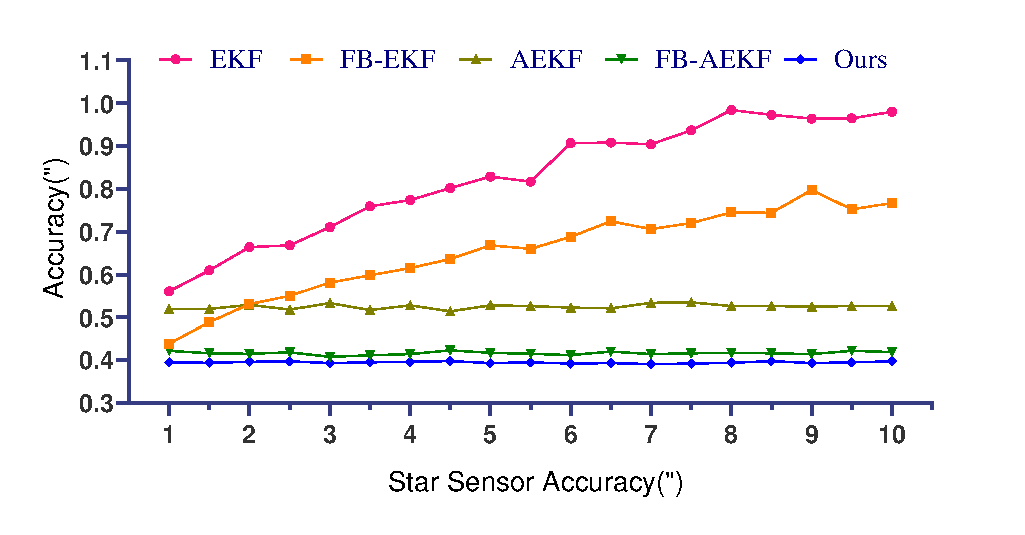
\includegraphics[width=\linewidth]{pic/exp1-roll.eps}
			\caption{RMS of roll angle}
			\label{fig:roll}
		\end{minipage}%	
		\begin{minipage}[t]{0.5\linewidth}
			\centering
			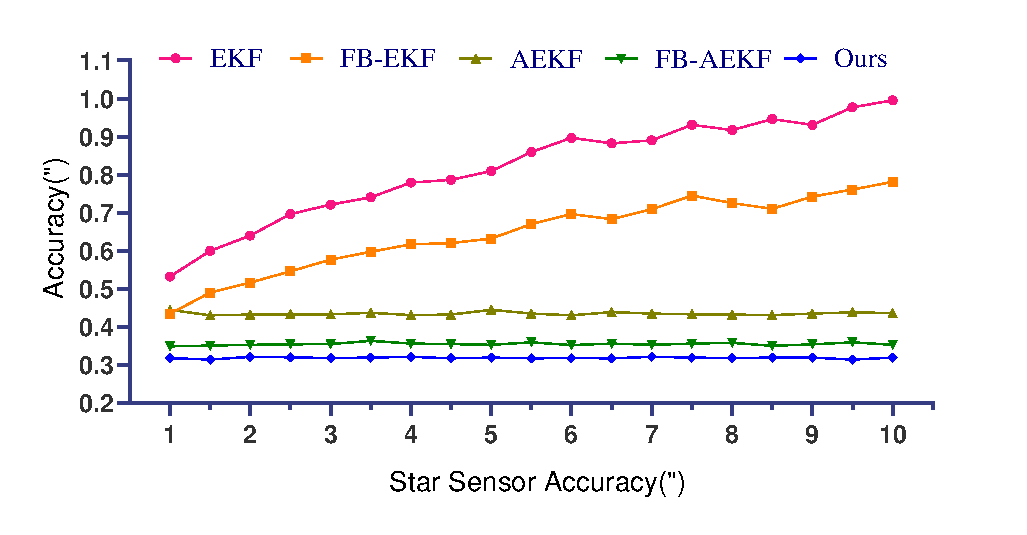
\includegraphics[width=\linewidth]{pic/exp1-pitch.eps}
			\caption{RMS of pitch angle}
			\label{fig:pitch}
		\end{minipage}
		
		\begin{minipage}[t]{\linewidth}
			\centering
			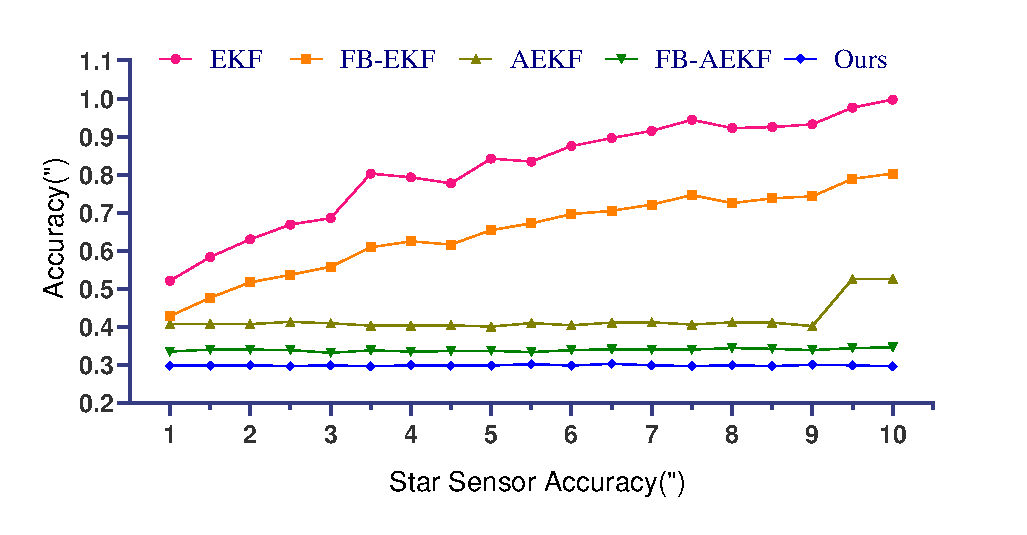
\includegraphics[width=0.5\linewidth]{pic/exp1-yaw.eps}
			\caption{RMS of yaw angle}
			\label{fig:yaw}
		\end{minipage}
	\end{figure}
	
	In this experiment, the training process of the algorithm in this paper uses only the AEKF test results with a prior error of $ 3'' $ for the star sensor. When the algorithm is used for online prediction, it achieves high accuracy and stable results in the range of $ 1.0''-10.0'' $, which proves that the ELM model has good generalization performance and is suitable for the case of inaccurate prior noise characteristics of the star sensor.
	
	\section{Conclusions}
	\label{sec:con}
	
	In this paper, we propose a high-precision satellite attitude determination algorithm based on extreme learning machine network correction. The problem of linearization and discrete system error is adddressed, which in the Kalman filter-based attitude determination task. A comparison experiment is conducted using simulation data. The results show that the proposed method has improved the accuracy and stability compared with the traditional algorithm. This ELM-based algorithm with less computation and lower computational complexity. The proposed method provides a reference for further improving the accuracy and stability of satellite attitude determination, which has important practical significance.
	
	% References should be produced using the bibtex program from suitable
	% BiBTeX files (here: strings, refs, manuals). The IEEEbib.bst bibliography
	% style file from IEEE produces unsorted bibliography list.
	% -------------------------------------------------------------------------
	\bibliographystyle{IEEEbib}
	\bibliography{myrefs}
	
\end{document}
